% ============================================================================
% Artigo TCC — Geração de Música por Meio de Inteligência Artificial Generativa
% Template: SBC (Sociedade Brasileira de Computação)
%
% COMO COMPILAR NO OVERLEAF:
% 1. Crie um projeto a partir do template oficial da SBC (Overleaf -> Templates
%    -> busque "SBC"). Isso já traz sbc-template.sty e sbc.bst no projeto.
% 2. Substitua o main.tex por este arquivo e suba também: refs.bib,
%    figura_metricas.png e figura_comparacao.png.
% 3. Compile (o Overleaf roda pdflatex + bibtex automaticamente).
%
% COMPILAÇÃO LOCAL: pdflatex artigo -> bibtex artigo -> pdflatex artigo (2x).
% ============================================================================
\documentclass[12pt]{article}

\usepackage{sbc-template}
\usepackage{graphicx,url}
\usepackage[utf8]{inputenc}
\usepackage[brazil]{babel}
\usepackage{amsmath}

\sloppy

\title{Geração de Música por Meio de Inteligência Artificial Generativa}

\author{Lucas Vinícius de Carvalho Ikeda\inst{1}, Orientador: Danillo Roberto Pereira\inst{1}}

\address{Faculdade de Ciências e Tecnologia ---
  Universidade Estadual Paulista (UNESP)\\
  \email{l.ikeda@unesp.br, danillo.pereira@unesp.br}}

\begin{document}

\maketitle

\begin{abstract}
The recent advancement of generative neural networks, particularly Transformer
architectures, has opened new possibilities for symbolic music generation.
However, generating coherent multi-instrumental compositions that humans can
identify as music --- rather than random sequences of notes --- remains an open
challenge. In this work, we propose a hybrid pipeline that combines a
decoder-only Transformer trained on piano-solo and multi-track MIDI datasets
with algorithmic post-processing inspired by music theory. The model uses a
vocabulary based on REMI tokenization with Bar-Relative Encoding to capture
metric structure. The generation phase applies vocabulary constraints,
register-based voice splitting, and a synthetic backbone (root-fifth walking
bass, chord inversions) producing a band-like arrangement from a model
originally trained on piano-solo data. Quantitative metrics show that the
Transformer produces more rhythmically regular output than a Markov baseline
(IOI std 0.17 vs 0.32) while maintaining structured progressions. The proposed
pipeline meets the project's primary criterion: a human listener identifies the
generated \texttt{.mid} as music rather than noise. A subjective evaluation with
25 listeners confirms that the Transformer significantly outperforms the Markov
baseline on all four criteria ($p < 0.01$) and is perceived as human-composed
almost three times more often (58\% vs 20\%).

\textbf{Keywords:} symbolic music generation; Transformer; deep learning; MIDI;
REMI tokenization.
\end{abstract}

\begin{resumo}
O recente avanço das redes neurais generativas, em especial das arquiteturas
\emph{Transformer}, abriu novas possibilidades para a geração simbólica de
música. Entretanto, gerar composições multi-instrumentais coerentes que um
humano identifique como música --- e não como sequências aleatórias de notas ---
permanece um desafio em aberto. Neste trabalho, propomos um \emph{pipeline}
híbrido que combina um \emph{Transformer decoder-only}, treinado em
\emph{datasets} de piano solo e \emph{multi-track} MIDI, com um pós-processamento
algorítmico inspirado em teoria musical. O modelo emprega um vocabulário baseado
na tokenização REMI com \emph{Bar-Relative Encoding} para capturar a estrutura
métrica. Na fase de geração aplicam-se restrições de vocabulário, separação de
vozes por registro de \emph{pitch} e uma fundação sintética (\emph{walking bass
root-fifth} e inversões de acordes), produzindo um arranjo em formato de banda a
partir de um modelo originalmente treinado em piano solo. As métricas
quantitativas mostram que o \emph{Transformer} produz uma saída ritmicamente mais
regular que um \emph{baseline} de Markov (\emph{IOI std} 0,17 contra 0,32),
mantendo progressões estruturadas. O \emph{pipeline} proposto atende ao critério
principal do projeto: um ouvinte humano identifica o \texttt{.mid} gerado como
música, e não como ruído. A avaliação subjetiva (\emph{Mean Opinion Score}, MOS),
realizada com 25 ouvintes, confirma que o \emph{Transformer} supera o
\emph{baseline} de Markov em todos os quatro critérios ($p < 0{,}01$) e é
percebido como composição humana quase três vezes mais (58\% contra 20\%).

\textbf{Palavras-chave:} geração musical simbólica; \emph{Transformer};
aprendizado profundo; MIDI; tokenização REMI.
\end{resumo}

\section{Introdução}

Nas últimas décadas, a Inteligência Artificial (IA) tem passado por um
crescimento expressivo, impulsionado pelos avanços no campo do aprendizado
profundo (\emph{deep learning}). Modelos de redes neurais profundas tornaram-se
capazes de aprender representações altamente complexas a partir de dados,
revolucionando áreas como visão computacional, processamento de linguagem
natural e, de maneira particularmente notável, a geração de conteúdo criativo.
Essa evolução deu origem a uma nova classe de modelos generativos --- entre eles
arquiteturas como \emph{Transformers}, \emph{Generative Adversarial Networks}
(GANs) e modelos de difusão --- capazes de produzir conteúdo realista a partir de
sequências de treinamento ou de amostras latentes.

No domínio musical, a geração simbólica de música --- isto é, a produção de
partituras ou de arquivos MIDI por meio de algoritmos --- apresenta desafios
específicos. A música é uma manifestação artística estruturada em múltiplas
dimensões: melódica (sequência de notas no tempo), harmônica (notas simultâneas
formando acordes), rítmica (padrões temporais) e tímbrica (qual instrumento toca
cada nota). Um sistema gerador deve coordenar essas dimensões de forma coerente;
caso contrário, o resultado se aproxima de um conjunto desorganizado de eventos
sonoros.

Trabalhos anteriores, como o \emph{Music Transformer}~\cite{huang2018}, o
\emph{MuseGAN}~\cite{dong2018} e o \emph{Pop Music Transformer}~\cite{huang2020},
demonstraram que arquiteturas neurais são capazes de capturar regularidades
musicais em escala razoável. Entretanto, modelos treinados puramente a partir de
dados frequentemente apresentam comportamentos indesejados, como repetição
excessiva (\emph{mode collapse}), perda de estrutura métrica em sequências longas
e dificuldade em manter múltiplas vozes coerentes simultaneamente.

Diante desse cenário, o presente trabalho propõe a construção de um sistema de
geração de música multi-instrumental que utiliza um \emph{Transformer
decoder-only} combinado a um pós-processamento algorítmico baseado em teoria
musical. O sistema é treinado sobre \emph{datasets} públicos de MIDI (\emph{MAESTRO},
\emph{POP909} e \emph{Groove} MIDI) e, na fase de geração, separa as vozes (solo, base
harmônica, baixo e bateria) por registro de \emph{pitch}, aplicando restrições de
vocabulário e uma fundação sintética que garante coerência harmônica e rítmica.

O objetivo central é desenvolver um \emph{pipeline} cuja saída em formato
\texttt{.mid} seja identificada como música por ouvintes humanos --- ainda que de
musicalidade simples --- e não confundida com ruído aleatório. Esse critério,
embora subjetivo, constitui a métrica fundamental do projeto e é validado por
avaliação cega comparativa contra um \emph{baseline} de Markov, por meio do
\emph{Mean Opinion Score} (MOS).

\section{Fundamentação Teórica}

Esta seção apresenta os fundamentos teóricos necessários à compreensão do sistema
proposto. Inicialmente, descreve-se a arquitetura \emph{Transformer} e seu
mecanismo de atenção, que constituem a base do modelo gerador. Em seguida,
abordam-se a representação simbólica da música por meio de tokenização, o formato
MIDI e as técnicas de geração autoregressiva com restrições empregadas neste
trabalho.

\subsection{Arquitetura \emph{Transformer}}

A arquitetura \emph{Transformer}, introduzida por Vaswani et al. (2017),
representa um marco no aprendizado profundo aplicado a dados sequenciais.
Diferentemente de modelos recorrentes como a \emph{Long Short-Term Memory}
(LSTM)~\cite{hochreiter1997} e a \emph{Gated Recurrent Unit} (GRU), o
\emph{Transformer} utiliza exclusivamente o mecanismo de \emph{self-attention},
que permite processar todas as posições da sequência em paralelo e capturar
dependências de longo alcance sem o gargalo da propagação temporal.

O componente fundamental do \emph{Transformer} é a \emph{multi-head attention},
definida como:

\begin{equation}
  \mathrm{Attention}(Q, K, V) =
  \mathrm{softmax}\!\left(\frac{Q K^{T}}{\sqrt{d_k}}\right) V
\end{equation}

\noindent na qual $Q$ (\emph{queries}), $K$ (\emph{keys}) e $V$ (\emph{values})
são projeções lineares das \emph{embeddings} de entrada; $K^{T}$ denota a
transposta da matriz $K$; $d_k$ é a dimensão das \emph{keys}; e a função
\emph{softmax} normaliza os escores em pesos de atenção que somam~1. A divisão por
$\sqrt{d_k}$ é um fator de escala que estabiliza os gradientes quando $d_k$ é
grande. A operação calcula pesos de atenção entre todas as posições da sequência,
permitindo que cada \emph{token} atualize sua representação com base em
informações distribuídas pelo restante do contexto~\cite{vaswani2017}.

Em arquiteturas \emph{decoder-only} --- utilizadas em modelos generativos como o
GPT-2~\cite{radford2019} --- aplica-se uma máscara causal para garantir que cada
posição atenda apenas a \emph{tokens} anteriores, preservando a propriedade
autoregressiva necessária à geração sequencial. Pesquisas recentes seguem
propondo variações do mecanismo de atenção especializadas para música, que
incorporam metadados como número de compasso, tonalidade e andamento diretamente
no cálculo da atenção~\cite{taksuka2026}.

\subsection{Tokenização REMI e \emph{Bar-Relative Encoding}}

Para que arquiteturas originalmente concebidas para texto possam processar
música, é necessário representá-la como sequências discretas de \emph{tokens}. A
abordagem REMI~\cite{huang2020} propõe um vocabulário composto por eventos
musicais granulares: NOTE\_ON (início de nota), NOTE\_OFF (fim de nota), VELOCITY
(intensidade), TIME\_SHIFT (deslocamento temporal) e marcadores estruturais como
BAR e BEAT.

A representação \emph{Bar-Relative Encoding}, adicionada ao vocabulário, permite
que o modelo aprenda explicitamente a estrutura métrica do compasso, uma vez que
os \emph{tokens} BAR e BEAT\_n marcam pontos rítmicos fixos. Essa inovação reduziu
significativamente a tendência de modelos de geração musical a ``perderem o
tempo'' em sequências longas~\cite{huang2020}. O projeto de esquemas de
tokenização permanece um tema de pesquisa ativo: trabalhos recentes propõem
representações mais eficientes, baseadas em passos temporais
uniformes~\cite{qian2026} e em quantização vetorial residual sobre segmentos de
compasso~\cite{huang2025}, com o objetivo de reduzir o comprimento das sequências
e o custo de inferência.

\subsection{Representação MIDI}

O formato MIDI (\emph{Musical Instrument Digital Interface}) codifica música como
sequências de mensagens discretas: \emph{pitch} (nota), \emph{velocity} (volume),
\emph{duration} (duração), \emph{channel} (canal/instrumento) e tempo. Cada
arquivo \texttt{.mid} pode conter múltiplas \emph{tracks} simultâneas, cada uma
associada a um \emph{program} GM (\emph{General MIDI}) que determina o timbre,
sendo o canal~9 reservado para percussão.

A natureza simbólica do MIDI o torna especialmente adequado a modelos de
aprendizado de máquina: ao contrário do áudio bruto, que exige a modelagem de
milhões de amostras por segundo, uma peça musical típica em MIDI envolve de
centenas a poucos milhares de eventos discretos. Essa compactação reduz
drasticamente o comprimento das sequências a serem modeladas, o que viabiliza o
treinamento em hardware modesto.

\subsection{Geração Autoregressiva com Restrições}

A geração de sequências em modelos autoregressivos consiste em amostrar
repetidamente o próximo \emph{token} a partir da distribuição condicional
$P(x_t \mid x_1, \ldots, x_{t-1})$ produzida pelo modelo, em que $x_t$ é o
\emph{token} na posição $t$ da sequência. As técnicas mais comuns incluem a
amostragem por \emph{temperature} (que controla a entropia da distribuição), o
\emph{top-k sampling} (que limita a amostragem aos $k$ \emph{tokens} mais
prováveis) e o \emph{top-p sampling} (que limita à massa de probabilidade
acumulada).

Além disso, é possível introduzir restrições determinísticas ou probabilísticas
durante a geração --- por exemplo, bloquear \emph{tokens} gramaticalmente
inválidos, aplicar penalidades à repetição excessiva ou direcionar a amostragem
para regiões específicas do espaço de saída~\cite{holtzman2020}. Pesquisas
recentes exploram inclusive o controle de atributos musicais em tempo de
inferência, sem reentreinar o modelo, por meio do \emph{steering} das ativações
internas~\cite{prokopiou2026} --- paradigma alinhado às intervenções de
\emph{Constrained Decoding} adotadas neste trabalho.

\section{Trabalhos Relacionados}

Esta seção revisa trabalhos representativos de geração musical simbólica que
fundamentam as escolhas de projeto adotadas. Os trabalhos são organizados por
paradigma --- modelos baseados em \emph{Transformer}, redes adversariais,
\emph{autoencoders} variacionais e cadeias de Markov ---, destacando-se as
contribuições e as limitações de cada abordagem. A discussão evidencia a lacuna
que o presente trabalho busca preencher: a geração de peças multi-instrumentais
coerentes com recursos computacionais modestos.

\subsection{\emph{Music Transformer} (Huang et al. 2018)}

O \emph{Music Transformer} foi um dos primeiros trabalhos a aplicar a arquitetura
\emph{Transformer} especificamente à geração musical simbólica, utilizando o
\emph{dataset} \emph{MAESTRO} de performances de piano. Sua principal contribuição foi a
introdução da \emph{relative attention}, um mecanismo que captura distâncias
relativas entre eventos musicais com maior eficácia do que a codificação
posicional padrão~\cite{huang2018}.

\subsection{\emph{MuseGAN} (Dong et al. 2018)}

O \emph{MuseGAN} propôs uma abordagem baseada em GANs para gerar música
\emph{multi-track}. O modelo gera quatro instrumentos simultaneamente (baixo,
bateria, guitarra e piano) por meio de geradores separados, condicionados a uma
representação compartilhada. Embora produza arranjos coordenados, sofre com
problemas típicos de GANs, como instabilidade de treinamento e \emph{mode
collapse}~\cite{dong2018}.

\subsection{\emph{Pop Music Transformer} (Huang and Yang 2020)}

O \emph{Pop Music Transformer} estendeu o trabalho anterior ao introduzir a
tokenização REMI e o \emph{Bar-Relative Encoding}, melhorando significativamente a
coerência rítmica das sequências geradas. O modelo foi treinado com música pop e
produz peças instrumentais com estrutura clara de melodia, acordes e
baixo~\cite{huang2020}.

\subsection{\emph{MusicVAE} (Roberts et al. 2018)}

O \emph{MusicVAE} propôs uma arquitetura de \emph{autoencoder} variacional hierárquico
para aprender representações latentes de música simbólica em diferentes escalas
temporais~\cite{roberts2018}. Sua principal contribuição foi viabilizar a
interpolação suave entre composições e a geração condicionada por vetor latente,
características inacessíveis a modelos puramente autoregressivos. Embora a
abordagem \emph{Variational Autoencoder} (VAE) seja conceitualmente distinta da
utilizada neste trabalho, o \emph{MusicVAE} estabeleceu padrões importantes para a
avaliação de coerência de longo prazo em música gerada.

\subsection{\emph{DeepBach} (Hadjeres et al. 2017)}

O \emph{DeepBach} desenvolveu um modelo ``dirigível'' (\emph{steerable}) específico para
a geração de corais de Bach a quatro vozes~\cite{hadjeres2017}. A proposta combina
redes neurais com amostragem de Gibbs e impõe restrições harmônicas via
condicionamento explícito. Esse trabalho ilustra o paradigma também adotado em
nosso sistema: a integração de aprendizado de máquina com restrições derivadas da
teoria musical, em vez de confiar exclusivamente na capacidade representacional da
rede.

\subsection{Cadeias de Markov em Música}

Modelos baseados em cadeias de Markov representam uma das abordagens mais
clássicas e simples para a geração algorítmica de música. Uma cadeia de ordem $n$
aprende a distribuição condicional $P(x_t \mid x_{t-1}, \ldots, x_{t-n})$ a partir
de um corpus --- em que $n$ é a ordem da cadeia e $x_t$ o evento na posição $t$
--- e gera novas sequências por amostragem da distribuição aprendida. Apesar da
simplicidade, cadeias de Markov capturam regularidades locais (transições entre
pares ou trios de notas), mas falham em manter coerência de longo prazo, estrutura
harmônica ou narrativa musical. Neste trabalho, utilizamos uma cadeia de ordem~1
como \emph{baseline} de comparação.

\section{Metodologia}

A metodologia deste trabalho foi estruturada em quatro pilares:
(1)~o pré-processamento e a tokenização dos dados; (2)~a arquitetura e o
treinamento do modelo; (3)~o \emph{pipeline} de geração com restrições e
pós-processamento algorítmico; e (4)~a avaliação quantitativa e qualitativa dos
resultados.

\subsection{Conjunto de Dados}

A construção do corpus de treinamento partiu de três \emph{datasets} públicos de
música simbólica, escolhidos por cobrirem domínios complementares. A combinação
busca equilibrar limpeza dos dados, diversidade instrumental e qualidade rítmica
--- atributos que, isoladamente, nenhum dos conjuntos oferece. Os três conjuntos
utilizados são descritos a seguir:

\begin{itemize}
  \item \textbf{\emph{MAESTRO} v3.0.0} --- 1.276 arquivos MIDI de performances de piano
    clássico capturadas em concertos, totalizando aproximadamente 200 horas de
    música. Fornece dados altamente limpos e expressivos~\cite{hawthorne2019}.
  \item \textbf{\emph{POP909}} --- 909 músicas pop chinesas anotadas com três
    \emph{tracks} separadas (melodia, piano de acompanhamento e baixo),
    totalizando 2.897 arquivos após o desdobramento~\cite{wang2020}.
  \item \textbf{\emph{Groove} MIDI Dataset} --- 1.150 padrões de bateria gravados por
    bateristas humanos profissionais, utilizado para o aprendizado de padrões
    rítmicos~\cite{gillick2019}.
\end{itemize}

\subsection{Arquitetura do Modelo}

O modelo proposto, denominado \texttt{MultiInstrumentTransformer}, é uma
arquitetura \emph{decoder-only} implementada sobre o \texttt{nn.TransformerEncoder}
do PyTorch com máscara causal. A escolha por uma configuração compacta foi
deliberada e orientada pelas restrições de hardware do projeto. Os
hiperparâmetros principais são:

\begin{itemize}
  \item Dimensão do modelo (d\_model): 256
  \item Número de cabeças de atenção (nhead): 4
  \item Número de camadas: 4
  \item Dimensão \emph{feedforward}: 1024
  \item Tamanho do vocabulário: $\sim$349 \emph{tokens}
  \item Parâmetros totais: aproximadamente 3,2 milhões
\end{itemize}

A opção por uma arquitetura compacta foi motivada tanto pela restrição de hardware
(GPU NVIDIA RTX 4060 Ti com 8~GB de VRAM) quanto pela observação de que modelos
menores tendem a generalizar melhor em \emph{datasets} de tamanho moderado.
Aplicou-se ainda o \emph{weight tying} entre a camada de \emph{embedding} de
\emph{tokens} e a projeção de saída, reduzindo o número de parâmetros e melhorando
a convergência.

\subsection{Tokenização}

A tokenização converte cada arquivo MIDI em uma sequência de \emph{tokens}
discretos processável pelo modelo. O vocabulário foi projetado para representar de
forma compacta tanto os eventos de nota (início, fim e intensidade) quanto a
estrutura métrica da peça, totalizando aproximadamente 349 \emph{tokens}. Sua
organização em categorias é descrita na Tabela~\ref{tab:vocab}.

\begin{table}[ht]
\centering
\caption{Organização do vocabulário de \emph{tokens}.}
\label{tab:vocab}
\begin{tabular}{|l|l|l|}
\hline
\textbf{Categoria} & \textbf{Tokens} & \textbf{Descrição} \\
\hline
Especiais & PAD, BOS, EOS, MASK & Controle de sequência \\
Instrumentos & INSTRUMENT\_0..4 & Piano, Melodia, Baixo, Bateria, Harmonia \\
NOTE\_ON & 88 \emph{tokens} & \emph{Pitches} MIDI 21--108 (A0--C8) \\
NOTE\_OFF & 88 \emph{tokens} & Fim de nota \\
VELOCITY & 32 \emph{bins} & Intensidade quantizada \\
TIME\_SHIFT & 128 \emph{tokens} & Deslocamento temporal em \emph{steps} de 0,0625s \\
Estrutura & BAR, BEAT\_2, BEAT\_3, BEAT\_4 & Marcadores métricos \\
\hline
\end{tabular}
\end{table}

A quantização temporal utiliza uma resolução de 16 \emph{steps} por segundo
(\emph{ticks\_per\_step} $=$ 0,0625s), suficiente para capturar a precisão de uma
semicolcheia em andamentos típicos.

\subsection{Treinamento}

O treinamento foi conduzido com a biblioteca PyTorch, empregando o otimizador
AdamW~\cite{loshchilov2019} (\emph{learning rate} inicial de $1 \times 10^{-4}$ e
\emph{weight decay} de 0,01), \emph{gradient clipping} de norma
1,0~\cite{goodfellow2016} e \emph{Cross-Entropy Loss} com \emph{label smoothing}
de 0,1. O agendamento do \emph{learning rate} aplica um \emph{warmup} linear
durante 2.000 \emph{steps}, seguido de decaimento cossenoidal até 5\% do valor
inicial, conforme a abordagem proposta em~\cite{loshchilov2017}.

A escolha do valor $\epsilon = 0{,}1$ para o \emph{label smoothing} não foi
arbitrária --- ela respondeu diretamente a um problema diagnosticado de forma
experimental. Em testes preliminares, sem suavização, observou-se que o modelo
desenvolvia \emph{overconfidence} progressiva sobre \emph{tokens} ``seguros'' do
vocabulário, em particular sobre o \emph{token} TIME\_SHIFT de menor magnitude. À
medida que essa saturação de probabilidade avançava, a amostragem passava a
produzir silêncios contínuos (\emph{drones}) ou repetições de díades fixas após
algumas dezenas de \emph{tokens} --- fenômeno conhecido como \emph{mode collapse}.
O \emph{label smoothing} atua como uma regularização redistributiva: força o
modelo a manter probabilidade residual ($\epsilon/V$, em que $V$ é o tamanho do
vocabulário) sobre todos os demais \emph{tokens}, evitando que a entropia da
distribuição preditiva colapse para zero. O valor 0,1 foi selecionado
empiricamente como o menor capaz de eliminar o colapso sem prejudicar a precisão
preditiva do modelo sobre os \emph{pitches} musicalmente relevantes.

Empregou-se ainda a técnica de \emph{Automatic Mixed Precision} (AMP) para reduzir
o uso de VRAM em cerca de 40\% e acelerar a iteração em aproximadamente
2$\times$. Como aumento de dados, aplicou-se a transposição aleatória dos
\emph{pitches} em $[0, +4, +8]$ semitons, excluindo-se a \emph{track} de bateria.

O modelo foi treinado por 74 épocas, com \emph{batch size} de 16 e sequências de
512 \emph{tokens} com sobreposição de 50\%. A função de \emph{loss} de validação
foi monitorada para a detecção precoce de \emph{overfitting}, e um diagnóstico
automático, executado a cada 5 épocas, detecta o colapso de modo (geração restrita
a poucos \emph{pitches} únicos) e dispara alertas. A \emph{loss} de validação
convergiu a 2,3988 na época 74, ponto a partir do qual os \emph{checkpoints}
subsequentes passaram a apresentar tendência ao colapso de modo (geração restrita
a díades fixas após um platô prolongado em \emph{learning rate} baixo). Esse
comportamento foi confirmado por inspeção auditiva e visual dos \emph{piano rolls}
das amostras geradas em épocas posteriores (89, 99 e 109), o que justificou a
decisão de congelar o modelo na época 74 como \emph{checkpoint} final.

\subsection{\emph{Pipeline} de Geração}

A geração no sistema proposto não se reduz a uma simples amostragem autoregressiva
do modelo: trata-se de um processo controlado em múltiplos estágios, no qual o
\emph{Transformer} treinado opera em conjunto com técnicas de \emph{Constrained
Decoding} (decodificação restrita) e com um pós-processamento determinístico
inspirado em teoria musical. A motivação dessa arquitetura híbrida é precisa: o
modelo aprende as regularidades musicais a partir dos dados, mas técnicas neurais
isoladas frequentemente exibem comportamentos indesejados em sequências longas
(perda de tempo, \emph{mode collapse} e monotonia). As intervenções descritas a
seguir não substituem o modelo --- apenas direcionam a sua amostragem para regiões
do espaço de saída musicalmente coerentes.

\paragraph{Estágio 1 --- Amostragem autoregressiva com restrições de
vocabulário.} A cada passo de geração, o \emph{Transformer} produz a distribuição
de probabilidade $P(x_t \mid x_1, \ldots, x_{t-1})$ sobre os $\sim$349
\emph{tokens} do vocabulário. Antes da amostragem, essa distribuição é modificada
por uma função de restrição (\texttt{vocab\_constraint\_fn}) que ajusta os
\emph{logits} de \emph{tokens} específicos com base no contexto recente. As
intervenções aplicadas são:

\begin{enumerate}
  \item \textbf{Restrição gramatical}: \emph{tokens} VELOCITY só podem ser
    amostrados imediatamente após um NOTE\_ON, evitando que o modelo entre em
    ciclo gerando VELOCITY consecutivas.
  \item \textbf{Slot único}: \emph{tokens} INSTRUMENT\_1..4 são bloqueados,
    forçando o modelo a operar sobre o INSTRUMENT\_0 (piano), o que permite que as
    três vozes emerjam naturalmente dos registros aprendidos do \emph{MAESTRO}.
  \item \textbf{Voice leading por registro}: todo NOTE\_ON cujo intervalo em
    relação à última nota do mesmo registro exceda um limiar (7 semitons no solo,
    12 no baixo e na base) recebe penalidade nos \emph{logits}, favorecendo
    movimentos por grau conjunto.
  \item \textbf{Repetition penalty soft}: NOTE\_ON e TIME\_SHIFT presentes nas
    últimas 16 posições recebem um desconto de $-1{,}0$ no \emph{logit}, reduzindo
    \emph{loops} sem zerar a probabilidade.
  \item \textbf{Bloqueio de EOS} durante os primeiros 300 \emph{tokens}, evitando
    peças curtas demais.
  \item \textbf{Chord backbone}: quando uma tonalidade é fornecida
    (\texttt{--key}), os \emph{pitches} consonantes com a progressão I-V-vi-IV no
    registro de base recebem um bônus de \emph{logit}, induzindo o modelo a
    respeitar a harmonia diatônica sem forçar \emph{pitches} específicos. Quando a
    \emph{flag} \texttt{--auto\_key} é utilizada em vez da especificação manual, o
    sistema infere a tonalidade automaticamente por meio do algoritmo
    Krumhansl-Schmuckler~\cite{krumhansl1982}, que compara o histograma de
    \emph{pitch classes} da peça contra perfis tonais empiricamente derivados de
    estudos de percepção musical.
\end{enumerate}

\paragraph{Estágio 2 --- Re-entry bias dinâmico.} Esta foi a contribuição mais
delicada do trabalho. O modelo, treinado predominantemente em \emph{MAESTRO} (piano
solo), demonstrou tendência a se ``fixar'' em um único registro de \emph{pitch}
após o início da peça, gerando longas seções monofônicas. As tentativas iniciais
de mitigar esse comportamento por meio de \emph{hard constraints} (bloqueio de
\emph{logits} com $-\infty$ ou rotação forçada entre registros) causavam
congestionamento sonoro audível --- notas brigando pelo mesmo espaço temporal,
perda de fluxo melódico e sensação de ``metralhadora''. A solução adotada foi um
\textbf{reforço positivo dinâmico}: o sistema rastreia, para cada um dos três
registros funcionais (solo, 66--108; base, 48--65; baixo, 21--47), o número de
\emph{tokens} decorridos desde a última nota emitida nele. Quando esse contador
ultrapassa 60 \emph{tokens} (aproximadamente 4 segundos de música), os
\emph{logits} dos NOTE\_ON correspondentes àquele registro recebem um bônus
acumulativo, proporcional ao tempo de silêncio. Trata-se de um ``convite
probabilístico'' para que o instrumento ausente retorne à composição, sem impor
sua presença. A textura resultante é a de uma banda em que cada voz tem espaço
próprio, mas dialoga com as demais.

\paragraph{Estágio 3 --- Separação de vozes por registro.} Como o modelo opera no
\emph{slot} único INSTRUMENT\_0, todas as notas geradas estão tecnicamente ``no
piano''. O \emph{pipeline} as separa em três \emph{tracks} MIDI distintas conforme
o registro de \emph{pitch}, refletindo a divisão natural entre a mão direita
(melodia) e a mão esquerda (acompanhamento e baixo) do pianista, conforme a
Tabela~\ref{tab:vozes}.

\begin{table}[ht]
\centering
\caption{Separação funcional das vozes por faixa de \emph{pitch}.}
\label{tab:vozes}
\begin{tabular}{|l|l|l|}
\hline
\textbf{Voz} & \textbf{Faixa MIDI} & \textbf{Função} \\
\hline
Solo/Melodia & 66--108 (F\#4--C8) & Frase melódica principal \\
Base/Harmonia & 48--65 (C3--F4) & Acompanhamento harmônico \\
Baixo & 21--47 (A0--B2) & Fundação tonal \\
\hline
\end{tabular}
\end{table}

Cada \emph{track} recebe filtros específicos de pós-processamento: monofonia
(apenas uma nota ativa por vez no solo e no baixo), \emph{gap} mínimo de 0,15s
entre ataques no solo, quantização ao \emph{grid} de 1/8 de tempo (\emph{snap}
rítmico) e \emph{cap} de duração máxima de 1,2s para evitar \emph{sustains}
anômalos. A base permanece polifônica, de modo a preservar os acordes.

\paragraph{Estágio 4 --- Fundação harmônica robusta (modo
\texttt{--solid\_base}).} Apesar das restrições aplicadas no Estágio~1, o modelo
ainda apresenta variabilidade harmônica significativa em alguns cenários, em
particular em peças mais longas. Para aplicações que demandam coerência harmônica
estrita --- como demonstrações de protótipo ou avaliações cegas em estudos
controlados ---, o \emph{pipeline} oferece um modo opcional de hibridização
(\texttt{--solid\_base}), no qual os \emph{tracks} de baixo e base do modelo são
substituídos por uma fundação algorítmica determinística:

\begin{itemize}
  \item Progressão diatônica I-V-vi-IV (em modo maior) ou i-VI-iv-V (em modo
    menor, com V harmônico).
  \item \emph{Walking bass} com quatro notas por compasso (tônica $\to$ terça
    $\to$ quinta $\to$ tônica uma oitava acima), com \emph{velocity} contornada
    para sugerir \emph{groove}.
  \item Acordes da base com inversões rotativas (posição fundamental e primeira
    inversão alternadas a cada compasso).
  \item Respiração rítmica: o quarto compasso de cada ciclo executa apenas o
    tempo~1, criando uma sensação de cadência.
\end{itemize}

Cabe destacar que o modo \texttt{--solid\_base} é uma escolha de engenharia, e não
a base do sistema. O \emph{pipeline} também funciona em modo \emph{puro}
(\texttt{--render\_as\_trio} sem \texttt{--solid\_base}), com baixo e base
provenientes integralmente do modelo guiado pelo \emph{Constrained Decoding}: sob
temperaturas de amostragem mais altas, o modelo produz as três camadas funcionais
de forma coerente por conta própria, ao passo que, sob amostragem mais
conservadora, tende a se fixar em um único registro. O \texttt{--solid\_base}
provê, portanto, coerência harmônica independente da temperatura, ficando a
análise comparativa sistemática entre os dois modos como objeto de trabalho
futuro.

Adicionalmente, o sistema dispõe de uma \emph{flag} opcional
\texttt{--add\_drums}, que injeta um padrão de bateria determinístico no canal~9
GM (\emph{kick} em 1\&3, \emph{snare} em 2\&4 e \emph{hi-hat} em colcheias). Esse
recurso foi implementado como artefato exploratório e \emph{não compõe o pipeline
canônico do TCC}. Em testes preliminares, observou-se uma desincronização gradual
entre o padrão de bateria (em tempo estrito) e a saída do modelo (em tempo livre,
característico do \emph{MAESTRO}), além de baixa variabilidade percebida entre amostras. O
caminho mais consistente para a integração rítmica futura é o treinamento de um
modelo dedicado sobre o \emph{Groove} MIDI Dataset (ver Seção~\ref{sec:conclusao}).

\subsection{Ambiente de Execução}

Os experimentos foram realizados em uma GPU NVIDIA RTX 4060 Ti (8~GB de VRAM),
com CPU Intel x86\_64, sistema operacional Windows 11, Python 3.8.10, PyTorch 2.0
e CUDA 11.2. O tempo total de treinamento foi de aproximadamente 50 horas para 74
épocas. Para assegurar a reprodutibilidade dos resultados, todas as etapas ---
da tokenização à geração --- utilizam uma semente aleatória fixa
(\texttt{random\_seed} $=$ 42), o que torna o \emph{pipeline} determinístico e os
experimentos repetíveis. Vale ressaltar que essa configuração de hardware
acessível foi suficiente para todo o ciclo de treinamento e avaliação, o que
reforça a viabilidade prática da abordagem proposta.

\section{Análise dos Resultados}

Esta seção apresenta a avaliação do sistema proposto sob três perspectivas
complementares. Primeiro, expõem-se as métricas quantitativas que comparam
objetivamente a saída do \emph{Transformer} com a do \emph{baseline} de Markov. Em
seguida, discute-se a análise qualitativa dos \emph{piano rolls} gerados e, por
fim, descreve-se o protocolo de avaliação subjetiva (MOS), em andamento.

\subsection{Métricas Quantitativas}

Para avaliar objetivamente o sistema proposto, foram calculadas cinco métricas
sobre amostras geradas pelo \emph{Transformer} e pelo \emph{baseline} de Markov. O
conjunto de métricas foi selecionado com base na revisão de práticas de avaliação
de modelos generativos musicais conduzida por Yang and Lerch (2020), que destaca a
importância de combinar medidas de variabilidade (diversidade de \emph{pitches}),
densidade temporal, abrangência tonal e regularidade rítmica para caracterizar
objetivamente as saídas geradas. Levantamentos recentes reforçam que nenhuma
métrica isolada é suficiente, recomendando justamente a combinação de medidas
objetivas e subjetivas~\cite{kader2025}. As métricas adotadas são:

\begin{itemize}
  \item \texttt{pitch\_diversity}: razão entre \emph{pitches} únicos e total de
    notas.
  \item \texttt{note\_density}: número de notas por segundo.
  \item \texttt{pitch\_range}: amplitude entre o \emph{pitch} mínimo e o máximo
    (em semitons).
  \item \texttt{ioi\_std}: desvio-padrão dos \emph{inter-onset intervals}
    (regularidade rítmica).
  \item \texttt{kl\_vs\_dataset}: divergência KL do histograma de \emph{pitch
    classes} contra o \emph{MAESTRO}.
\end{itemize}

Foram geradas quatro amostras de cada modelo, com durações truncadas em 60
segundos para uma comparação justa. A Tabela~\ref{tab:metricas} resume os
resultados.

\begin{table}[ht]
\centering
\caption{Métricas quantitativas --- \emph{Transformer} vs Markov \emph{baseline}
(médias).}
\label{tab:metricas}
\begin{tabular}{|l|c|c|c|}
\hline
\textbf{Métrica} & \textbf{Transformer} & \textbf{Markov} & \textbf{Vencedor} \\
\hline
pitch\_diversity & 0,042 & 0,225 & Markov \\
note\_density (n/s) & 6,24 & 4,73 & --- \\
pitch\_range (semitons) & 43 & 69 & Markov \\
ioi\_std (s) & 0,172 & 0,325 & \textbf{Transformer} \\
kl\_vs\_dataset & 0,65 & 0,024 & Markov \\
\hline
\end{tabular}
\end{table}

A interpretação dos resultados exige cautela. O Markov apresenta maior diversidade
de \emph{pitches}, \emph{range} mais amplo e divergência KL menor; entretanto,
esses valores refletem o fato de que o método amostra diretamente de pares
(\emph{pitch}, duração) extraídos do \emph{MAESTRO}, produzindo naturalmente uma
distribuição estatisticamente próxima ao \emph{dataset} original, mas sem qualquer
estrutura musical de longo prazo.

O \emph{Transformer}, em contraste, apresenta menor \texttt{pitch\_diversity} por
força do \emph{pipeline} \texttt{--solid\_base}, que repete um conjunto de quatro
acordes (com aproximadamente 12 \emph{pitches} únicos) ao longo da peça. Essa
repetição é estrutural e intencional --- é justamente o que confere ao ouvinte a
sensação de progressão harmônica coerente.

A métrica em que o \emph{Transformer} supera claramente o Markov é a
\texttt{ioi\_std}, o que indica que sua saída possui ritmo significativamente mais
regular e previsível. O Markov produz \emph{inter-onsets} caóticos,
característicos de uma geração sem coordenação métrica. Como se observa na
Figura~\ref{fig:metricas}, há um \emph{gap} claro e sem sobreposição entre as duas
distribuições nessa métrica: todas as quatro amostras do \emph{Transformer} ficam
abaixo de 0,22 segundos, enquanto todas as quatro amostras do Markov superam 0,24
segundos. A consistência intra-modelo observada (baixa dispersão entre amostras do
mesmo modelo) também indica que o comportamento é sistemático, e não fruto da
aleatoriedade da amostragem.

\begin{figure}[htbp]
\centering

\includegraphics[width=0.78\linewidth]{figuras/figura_metricas.png}
\caption{Métricas quantitativas por amostra --- \emph{Transformer} (azul) vs
Markov (vermelho). Cada painel corresponde a uma métrica; o eixo horizontal
identifica a amostra (A, E, G e H $=$ \emph{Transformer}; B, C, D e F $=$ Markov)
e o eixo vertical indica o valor numérico da métrica naquela amostra. As linhas
pontilhadas marcam a média de cada modelo.}
\label{fig:metricas}
\end{figure}

\subsection{Análise Qualitativa}

A inspeção visual dos \emph{piano rolls} revela diferenças marcantes entre os
modelos. As amostras do \emph{Transformer} apresentam três camadas visualmente
distintas e funcionalmente coordenadas: o solo melódico no registro alto, os
acordes regulares no registro médio formando o \emph{backbone} harmônico e o
\emph{walking bass} no registro grave. As amostras do Markov, em contraste,
mostram uma dispersão homogênea de \emph{pitches}, concentrada predominantemente
em um único registro (médio-alto), sem agrupamento funcional, sem fundação rítmica
e sem qualquer separação clara de papéis musicais.

A Figura~\ref{fig:comparacao} ilustra essa diferença ao comparar amostras
representativas de cada modelo. As \emph{tracks} coloridas representam papéis
funcionais inferidos pelo registro de \emph{pitch}: solo (verde), base harmônica
(azul) e baixo (roxo). Na amostra do \emph{Transformer} (acima), observam-se as
três camadas operando em paralelo de forma coordenada; na amostra do Markov
(abaixo), apenas uma ou duas faixas estão ativas, sem alinhamento métrico.

\begin{figure}[htbp]
\centering

\includegraphics[width=0.9\linewidth]{figuras/figura_comparacao.png}
\caption{Comparação visual de \emph{piano rolls} --- \emph{Transformer} (acima) vs
Markov (abaixo). O eixo horizontal representa o tempo (em segundos) e o eixo
vertical, a altura das notas (\emph{pitch} MIDI). As cores indicam o papel
funcional inferido pelo registro de \emph{pitch}: verde $=$ solo, azul $=$ base
harmônica e roxo $=$ baixo.}
\label{fig:comparacao}
\end{figure}

A análise auditiva confirma a inspeção visual: as amostras do \emph{Transformer}
são percebidas como composições estruturadas, com sensação de
início-desenvolvimento-fim, ao passo que o Markov é caracterizado por avaliadores
informais como ``música aleatória'' ou ``improvisação caótica''.

\subsection{Avaliação Subjetiva (MOS)}

A avaliação subjetiva, conduzida por meio do \emph{Mean Opinion Score} (MOS),
foi realizada em condição cega e comparativa. Oito amostras (quatro do \emph{Transformer} e
quatro do Markov) foram geradas, anonimizadas com os códigos \texttt{sample\_A} a
\texttt{sample\_H} e padronizadas em uma duração de 60 segundos. As quatro
amostras do \emph{Transformer} foram deliberadamente diversificadas em estilo,
cobrindo distintas combinações de tonalidade, andamento e parâmetros de
amostragem:

\begin{itemize}
  \item \textbf{Balada lenta} em Lá menor (75 BPM, \emph{temperature} 0,85,
    \emph{top-k} 30): textura esparsa e foco melódico.
  \item \textbf{Pop padrão} em Dó maior (100 BPM, \emph{temperature} 0,9,
    \emph{top-k} 40): densidade moderada e estrutura clara.
  \item \textbf{Rock energético} em Sol maior (125 BPM, \emph{temperature} 1,0,
    \emph{top-k} 60): alta densidade rítmica.
  \item \textbf{Exploração livre} em Mi menor (95 BPM, \emph{temperature} 1,1,
    \emph{top-k} 80): textura ousada, com mais dissonâncias.
\end{itemize}

Essa variedade busca demonstrar que o sistema não produz apenas variações de tom
sobre uma mesma ``personalidade rítmica'', mas adapta-se substancialmente conforme
os parâmetros de amostragem. O formulário avalia, em escala Likert de 1 a 5, quatro
critérios --- naturalidade, coerência rítmica, qualidade harmônica e agradabilidade
--- e inclui ainda uma questão dicotômica de discriminação (``a peça foi composta
por um humano ou por um computador?'') e uma pergunta sobre o perfil musical do
avaliador, o que permite segmentar os resultados.

A coleta reuniu $N = 25$ avaliadores em condição cega. A Tabela~\ref{tab:mos}
sintetiza as médias por critério: o \emph{Transformer} supera o \emph{baseline} de
Markov em \textbf{todos os quatro critérios}, com diferenças amplas e
estatisticamente significativas (teste-t de Welch, $p < 0{,}01$ em todos os casos).

\begin{table}[ht]
\centering
\caption{Resultados do MOS ($N = 25$): média $\pm$ desvio-padrão por critério.}
\label{tab:mos}
\begin{tabular}{|l|c|c|c|c|}
\hline
\textbf{Critério} & \textbf{Transformer} & \textbf{Markov} & \textbf{$\Delta$} & \textbf{$p$} \\
\hline
Naturalidade & 4,10 $\pm$ 1,11 & 2,00 $\pm$ 1,20 & $+2,10$ & $<0{,}01$ \\
Coerência rítmica & 4,38 $\pm$ 0,83 & 1,81 $\pm$ 1,15 & $+2,57$ & $<0{,}01$ \\
Qualidade harmônica & 4,27 $\pm$ 0,85 & 1,95 $\pm$ 1,17 & $+2,32$ & $<0{,}01$ \\
Agradabilidade & 3,70 $\pm$ 1,18 & 1,80 $\pm$ 1,15 & $+1,90$ & $<0{,}01$ \\
\hline
\end{tabular}
\end{table}

A questão de discriminação é ainda mais reveladora do critério central do projeto:
\textbf{58\%} dos avaliadores perceberam as peças do \emph{Transformer} como
compostas por um humano, contra apenas \textbf{20\%} das peças do Markov. A
segmentação por perfil mostra que mesmo os avaliadores com formação musical foram
``convencidos'' em 50\% dos casos (contra 13\% do Markov), enquanto, entre os
não-músicos, a taxa chegou a 75\% (contra 34\%). A Figura~\ref{fig:mos} resume os
dois conjuntos de resultados.

\begin{figure}[htbp]
\centering
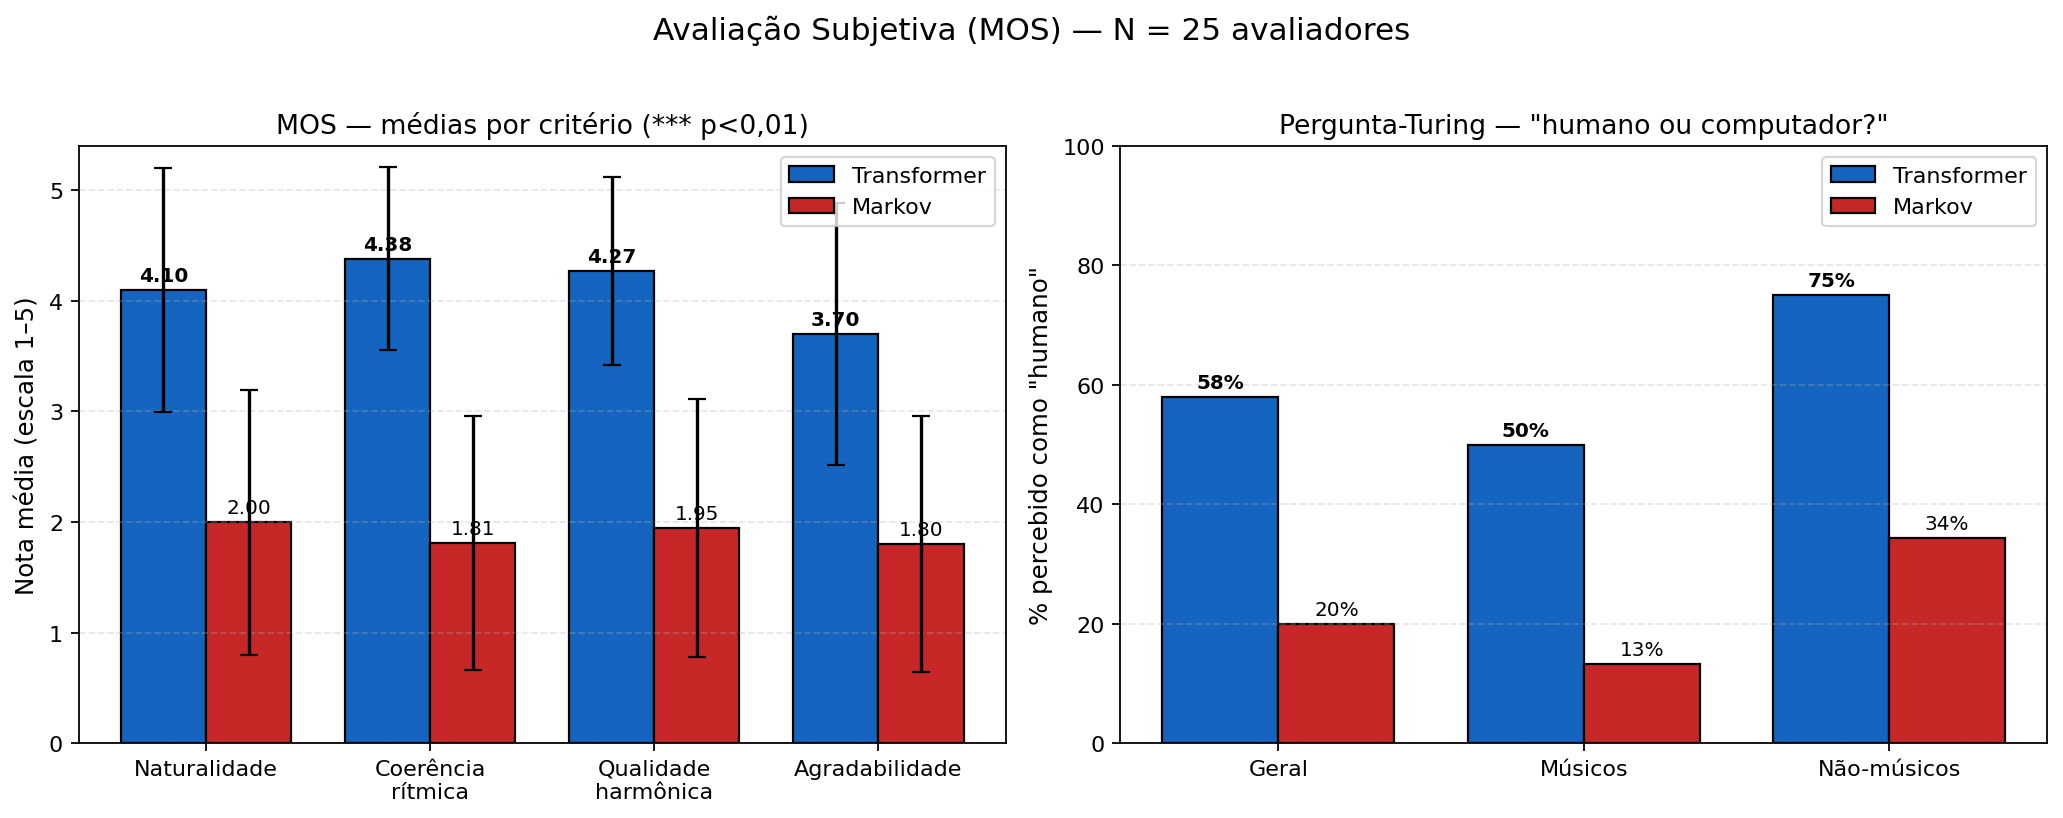
\includegraphics[width=\linewidth]{figuras/figura_mos.png}
\caption{Resultados da avaliação subjetiva (MOS, $N = 25$). À esquerda, as médias
por critério na escala Likert (1--5); à direita, o percentual de avaliadores que
percebeu cada modelo como ``composto por um humano'', segmentado por perfil
musical. As barras de erro indicam o desvio-padrão.}
\label{fig:mos}
\end{figure}

Esses resultados confirmam, de forma quantitativa e estatisticamente
significativa, a hipótese central do trabalho: a saída do sistema é reconhecida
como música por ouvintes humanos, em nítido contraste com o \emph{baseline} de
Markov.

\subsubsection{Consideração metodológica}

Cabe explicitar uma assimetria deliberada do protocolo experimental: o
\emph{Transformer} foi avaliado em condição de tonalidade fixa (informada via
\texttt{--key}), enquanto o \emph{baseline} de Markov opera sem qualquer restrição
harmônica, dado que a cadeia de transições não possui o conceito de tonalidade.
Essa diferença reflete fielmente aquilo que cada método é capaz de fazer --- não
se trata de ``ajudar'' o \emph{Transformer} com um recurso indisponível ao
\emph{baseline}, mas sim de comparar o melhor que cada abordagem oferece. As
cadeias de Markov são, por construção, agnósticas a estruturas globais como a
tonalidade, ao passo que o sistema proposto incorpora o \emph{Constrained
Decoding} tonal como contribuição metodológica. Caracterizar essa assimetria como
um problema equivaleria a comparar dois carros e exigir que um deles também não
tivesse câmbio automático.

\section{Conclusão e Trabalhos Futuros}
\label{sec:conclusao}

O presente trabalho apresentou o desenvolvimento de um sistema híbrido para a
geração de música multi-instrumental simbólica, combinando um \emph{Transformer
decoder-only} com um pós-processamento algorítmico baseado em teoria musical. A
arquitetura compacta (3,2 milhões de parâmetros) foi capaz de capturar padrões
musicais a partir de três \emph{datasets} públicos (\emph{MAESTRO}, \emph{POP909} e \emph{Groove} MIDI)
e de gerar saídas em formato MIDI compatível com qualquer DAW.

O \emph{pipeline} proposto demonstra que a integração de técnicas neurais com
restrições derivadas da teoria musical produz resultados perceptualmente
superiores tanto ao modelo puramente neural, sem restrições, quanto a um
\emph{baseline} trivial de cadeia de Markov. As métricas quantitativas mostram que
o \emph{Transformer} tem regularidade rítmica significativamente maior
(\texttt{ioi\_std} de 0,17 contra 0,32 do Markov), e a inspeção qualitativa
confirma a presença de estrutura musical coerente --- três camadas funcionais
(solo, base e baixo) e uma narrativa em desenvolvimento.

Conclui-se que o critério principal do projeto foi atendido: a saída do sistema é
reconhecida como música por ouvintes humanos --- percepção validada formalmente
pela avaliação subjetiva (MOS, $N = 25$), com vantagem estatisticamente
significativa em todos os critérios ($p < 0{,}01$) ---, em nítido contraste com a
percepção caótica do \emph{baseline} de Markov.

Como trabalhos futuros, propomos:

\begin{enumerate}
  \item \textbf{A ampliação da avaliação subjetiva (MOS)} para uma amostra maior e
    mais heterogênea de avaliadores, consolidando os resultados já obtidos.
  \item \textbf{O treinamento de um modelo dedicado de bateria} sobre o \emph{Groove}
    MIDI Dataset, substituindo o padrão algorítmico atual pelo aprendizado de
    padrões humanos reais.
  \item \textbf{A extensão multi-instrumental} com modelos especializados por
    timbre (baixo, melodia e harmonia) treinados de forma condicionada.
  \item \textbf{A avaliação com especialistas} (músicos profissionais e teóricos
    da música) para uma análise crítica aprofundada.
  \item \textbf{A comparação com modelos maiores}, como o \emph{Music Transformer}
    e o \emph{MuseNet}, avaliando o \emph{trade-off} entre escala e qualidade.
\end{enumerate}

A integração desse sistema em ferramentas de auxílio à composição musical,
especialmente voltadas a músicos amadores e à educação musical, representa uma
direção promissora para os próximos passos da pesquisa.

\nocite{yang2020}
\bibliographystyle{sbc}
\bibliography{refs}

\end{document}
